\chapter{Método de trabajo y herramientas}
\label{chap:metodo}

\drop{E}{n} este capitulo se expone la metodología seguida para llevar a cabo el proyecto y se
justifica porque se considera el método más satisfactorio a la hora de implementar este
\acs{TFG}. Además, se seleccionan y nombran las diferentes herramientas utilizadas para el
desarrollo del mismo tanto \emph{software} como \emph{hardware}.

\section{Metodología de trabajo}
\label{sec:metodologia}

Al comenzar este \acs{TFG} sólo disponíamos de una idea general del sistema que queríamos
desarrollar. Puesto que los requisitos de los que disponíamos no eran detallados, se decidió optar
por un modelo de desarrollo \emph{evolutivo} para ir detallando las especificaciones a lo largo del
progreso del proyecto. En particular, el de \emph{prototipos desechables} o \emph{prototipado
  evolutivo}.

El desarrollo \emph{evolutivo} se basa en la idea de crear una implementación inicial,
exponerla a los comentarios del usuario y refinarla a través de las diferentes versiones hasta
conseguir un sistema adecuado~\cite{Sommerville14}.

En la Figura~\ref{fig:modelo-evolutivo} se muestra el diagrama de flujo seguido por un modelo
evolutivo en el que se puede ver como las actividades de especificación, desarrollo y validación se
realizan de forma concurrente con una rápida retroalimentación entre ellas.

\begin{figure}[!h]
  \begin{center}
    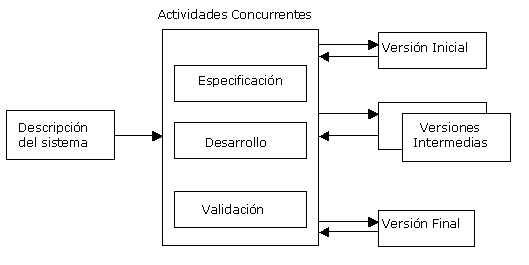
\includegraphics[width=0.75\textwidth]{/modelo-evolutivo.jpg}
    \caption{Diagrama de flujo del modelo de desarrollo evolutivo}
    \label{fig:modelo-evolutivo}
  \end{center}
\end{figure}

\subsection{Prototipado evolutivo}

El \emph{prototipado evolutivo} es un modelo de desarrollo de software basado en la realización de
prototipos funcionales hasta llegar a un producto final. Se parte de los requisitos mejor
comprendidos y con mayor prioridad, y se van definiendo los detalles conforme avanza el desarrollo
de las diferentes versiones.

Un cliente, a menudo, define un conjunto de objetivos generales para el \emph{software}, pero no
identifica los requisitos detallados de entrada, proceso o salida. De igual forma, el responsable
del desarrollo del \emph{software} puede no estar seguro de la eficacia de un algoritmo o de la
forma en que debería plantearse la \acs{IPO}. En estas y otras muchas situaciones, un paradigma de
construcción de prototipos puede ofrecer el mejor enfoque~\cite{Pressman10}.

El esquema general del \emph{prototipado evolutivo} se puede ver en la
Figura~\ref{fig:prototipo}. El paradigma comienza con una recolección de requisitos, es decir, el
desarrollador y el cliente definen los objetivos globales para el software, identifican los
requisitos conocidos y las áreas donde se necesita más definición. Entonces aparece un diseño rápido
centrado en los aspectos que serán visibles para el cliente y se construye un prototipo. Este
prototipo es evaluado por el cliente y se utiliza para refinar los requisitos del software. Esta
iteración se repite hasta llegar al resultado final.

\begin{figure}[!h]
  \begin{center}
    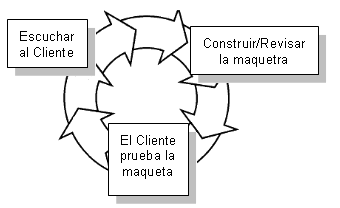
\includegraphics[width=0.6\textwidth]{/prototipo.png}
    \caption{Paradigma de construcción de prototipos}
    \label{fig:prototipo}
  \end{center}
\end{figure}

Entre las ventajas del uso del \emph{prototipado evolutivo} hay que destacar:

\begin{itemize}
  \item La continua obtención de prototipos permite al cliente observar y dirigir el desarrollo del
    \emph{software}.
  \item Las funcionalidades más importantes son desarrolladas en las primeras fases del proyecto y,
    por tanto, son las funcionalidades que más veces se ha probado su correcto funcionamiento.
  \item Como se evalúan prototipos intermedios, es más fácil comprobar si los requisitos planteados
    son correctos y viables.
\end{itemize}

Por otro lado, el \emph{prototipado evolutivo} también puede presentar algunas desventajas:

\begin{itemize}
  \item Resulta difícil estimar el coste final del proyecto debido al desconocimiento del número de
    iteraciones a realizar.
  \item Resulta muy difícil y costoso realizar cambios en la arquitectura del software.
\end{itemize}

Debido a estos problemas, aplicar el \emph{prototipado evolutivo} resulta muy complejo para grandes
proyectos pero resulta conveniente utilizarlo en sistemas pequeños y de tamaño medio como el
planteado en este \acs{TFG}. Para proyectos más grandes es recomendable utilizar un modelo híbrido
entre el modelo en cascada, para desarrollar las partes bien conocidas, y un enfoque evolutivo para
los aspectos que presenten mayor incertidumbre.

\section{Herramientas}

En esta sección se detallan las herramientas que han sido empeladas para la realización de este
\acs{TFG}, desde las necesarias para implementar el proyecto hasta las utilizadas para la
realización del documento.

\subsection{Hardware}
\label{sec:herramientasHardware}

Entre los medios necesarios para la puesta en marcha del sistema y la realización de las pruebas, se
han requerido los siguientes medios \emph{hardware}:

\begin{itemize}
  \item \textbf{Computador} Para el desarrollo de la aplicación y generar la documentación ha sido
    necesario empelar un ordenador de propósito general. En este caso se ha utilizado un ordenador
    portátil Asus X54H~\footnote{http://www.asus.com/Notebooks\_Ultrabooks/X54H/}.

  \item \textbf{Smartphones} Para las pruebas han sido necesarios varios \emph{smartphones} con
    diferentes versiones de Android. En todos se ha testeado tanto la aplicación de navegación como
    la aplicación para los complementos vibratorios:
    \begin{itemize}
      \item Nexus 5~\footnote{https://www.google.es/nexus/5/} con Android 5.0.1.
      \item Nexus One~\footnote{https://en.wikipedia.org/wiki/Nexus\_One} con Android 2.3.7.
      \item HTC Wildfire S~\footnote{https://en.wikipedia.org/wiki/HTC\_Wildfire\_S} con Android
        2.3.5.
    \end{itemize}

  \item \textbf{Smartwatch} Para realizar las pruebas para los complementos vibratorios con Android
    Wear se ha utilizado el LG G Watch
    R~\footnote{http://www.lg.com/es/wearables/lg-LGW110-g-watch-r}.

\end{itemize}

\subsection{Software}
\label{sec:herramientasSoftware}

A continuación se nombran las diferentes herramientas \emph{software} empleadas distinguiendo entre
diferentes categorías:

\subsubsection{Sistemas Operativos}

\begin{itemize}
  \item \textbf{Elementary OS}~\footnote{http://elementaryos.org/} Para la elaboración del trabajo
    se ha elegido esta distribución GNU/Linux como \acs{SO} del computador de
    desarrollo. Concretamente en su versión 0.3 \emph{Freya}.

  \item \textbf{Android}~\footnote{https://developer.android.com/index.html} Para desarrollar
    nuestra aplicación de navegación y algunos complementos vibratorios se seleccionó el \acs{SO}
    Android por ser la plataforma con más cuota de mercado y variedad de dispositivos.

  \item \textbf{Android Wear}~\footnote{https://developer.android.com/wear/index.html} Para
    desarrollar la aplicación de los complementos vibratorios se utilizó Android Wear ya que es la
    única plataforma de \emph{wearables} que nos permite acceder al vibrador incorporado.

\end{itemize}

\subsubsection{Herramientas de desarrollo}

\begin{itemize}
  \item \textbf{Android Studio}~\footnote{https://developer.android.com/sdk/index.html} Para el
    desarrollo de las aplicaciones del sistema de navegación desarrollado se selecciono Android
    Studio en su versión 1.0. Este entorno de desarrollo completamente orientado a Android y Android
    Wear.

  \item \textbf{Git}~\footnote{http://git-scm.com/} Para llevar un control de versiones y así
    mantener un historial de cambios, tanto en el desarrollo de las aplicaciones como en el
    desarrollo del proyecto, se ha utilizado Git. El servicio de repositorio empleado ha sido
    proporcionado por Bitbucket~\footnote{https://bitbucket.org/}.

\end{itemize}

\subsubsection{Librerías}

\begin{itemize}
  \item \textbf{Android
    support}~\footnote{https://developer.android.com/tools/support-library/index.html} Para lograr
    la compatibilidad entre las diferentes versiones de Android y de sus \acs{API} se utilizó esta
    librería suministrada por Google en su versión 4.21.0.3. También se utilizó \textbf{Android
      support appcompat} en su versión 7.21.0.3 para la compatibilidad del menú lateral.

  \item \textbf{Play services} Para la comunicación con los dispositivos \emph{wearables} se utilizó
    esta librería. Concretamente en su versión 6.5.87.

  \item \textbf{Commons Lang}~\footnote{https://commons.apache.org/proper/commons-lang/} Se
    utilizaron algunos de sus métodos del paquete \texttt{java.util}. Se empleó la versión 3.3.2.

  \item \textbf{Osmdroid}~\footnote{https://github.com/osmdroid/osmdroid} Para acceder a los mapas
    colaborativos de \acs{OSM} se utilizó esta librería en su versión 4.2.

  \item \textbf{Osmbonuspack}~\footnote{https://code.google.com/p/osmbonuspack/} Para realizar
    algunas acciones sobre los mapas de \acs{OSM} no disponibles en Osmdroid se utilizó esta
    librería en su versión 4.9.

  \item \textbf{Gson}~\footnote{https://code.google.com/p/google-gson/} Esta librería es la
    encargada de convertir objetos Java en su representación en JSON y viceversa. Es imprescindible
    para usar \emph{Osmdroid} y se utilizó la versión 2.3.1.

  \item \textbf{SLF4J}~\footnote{http://www.slf4j.org/} La librería Simple Logging Facade for Java
    (SLF4J) proporciona una \acs{API} de registro Java a través de patrón de fachada simple. Es
    imprescindible para el uso de \emph{Osmdroid} y se utilizó en la versión 1.5.8.
    %https://es.wikipedia.org/wiki/SLF4J

\end{itemize}

\subsubsection{Documentación y gráficos}

\begin{itemize}
  \item \textbf{Emacs}~\footnote{https://www.gnu.org/software/emacs/} El editor de texto
    «extensible, personalizable, auto-documentado y de tiempo real» ha sido utilizado en su versión
    23.4.1 para la elaboración de la documentación del \acs{TFG} utilizando los modos «latex» y
    «flyspell».

  \item \textbf{\LaTeX}~\footnote{http://www.latex-project.org/} Para la elaboración de este
    documento se ha empleado esta herramienta de creación de documentos profesionales. Más
    concretamente, la implementación \textit{TeX
      Live}~\footnote{\url{https://www.tug.org/texlive/}}.

  \item \textbf{BibTex}~\footnote{http://www.bibtex.org/} Se ha empleado esta herramienta destinada
    a la creación de referencias para documentos escritos en \LaTeX para hacer la bibliografía de
    este documento.

  \item \textbf{draw.io}~\footnote{https://www.draw.io/} Se ha utilizado esta aplicación web para
    crear la mayoría de diagramas de este documento.

  \item \textbf{Gimp}~\footnote{http://www.gimp.org/} Se ha usado este editor de imágenes avanzado
    para crear y retocar algunas imágenes del documento. Concretamente en su versión 2.8.14.

\end{itemize}

% Local Variables:
% TeX-master: "main.tex"
%  coding: utf-8
%  mode: latex
%  mode: flyspell
%  ispell-local-dictionary: "castellano8"
% End:
